\chapter{Конструкторский раздел}
\label{cha:design}

В данном разделе будет произведена разработка распараллеленного алгоритма Винограда.

\section{Функциональная модель}
На рисунке \ref{img:idef0} представлена функциональная модель IDEF0 уроня 1.
\begin{figure}
    \centering
    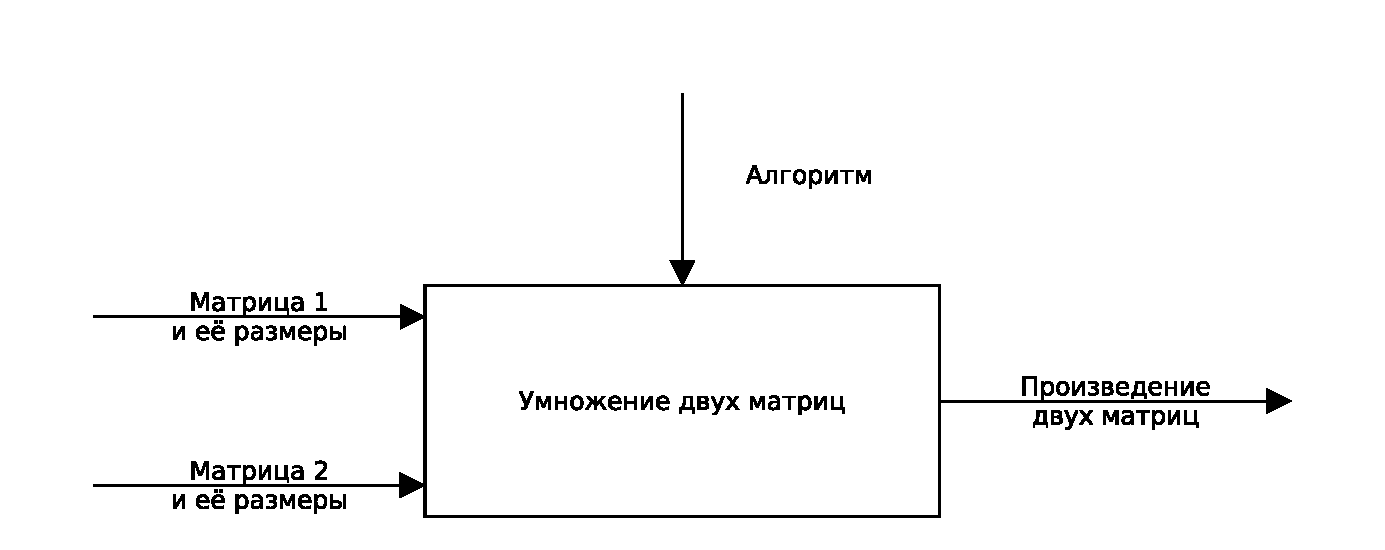
\includegraphics[scale=.7]{pdf/mainIdef0.pdf}
    \caption{функциональная модель IDEF0 уроня 1}
    \label{img:idef0}
\end{figure}

\section{Разработка алгоритмов}
Изобразим схемы алгоритма Винограда и распараллеленного алгоритма Винограда.

\subsection{Алгоритм Винограда}

На риснуках \ref{img:windograd1}, \ref{img:windograd2} изображена схема алгоритма Винограда.
\begin{figure}[H]
    \centering
    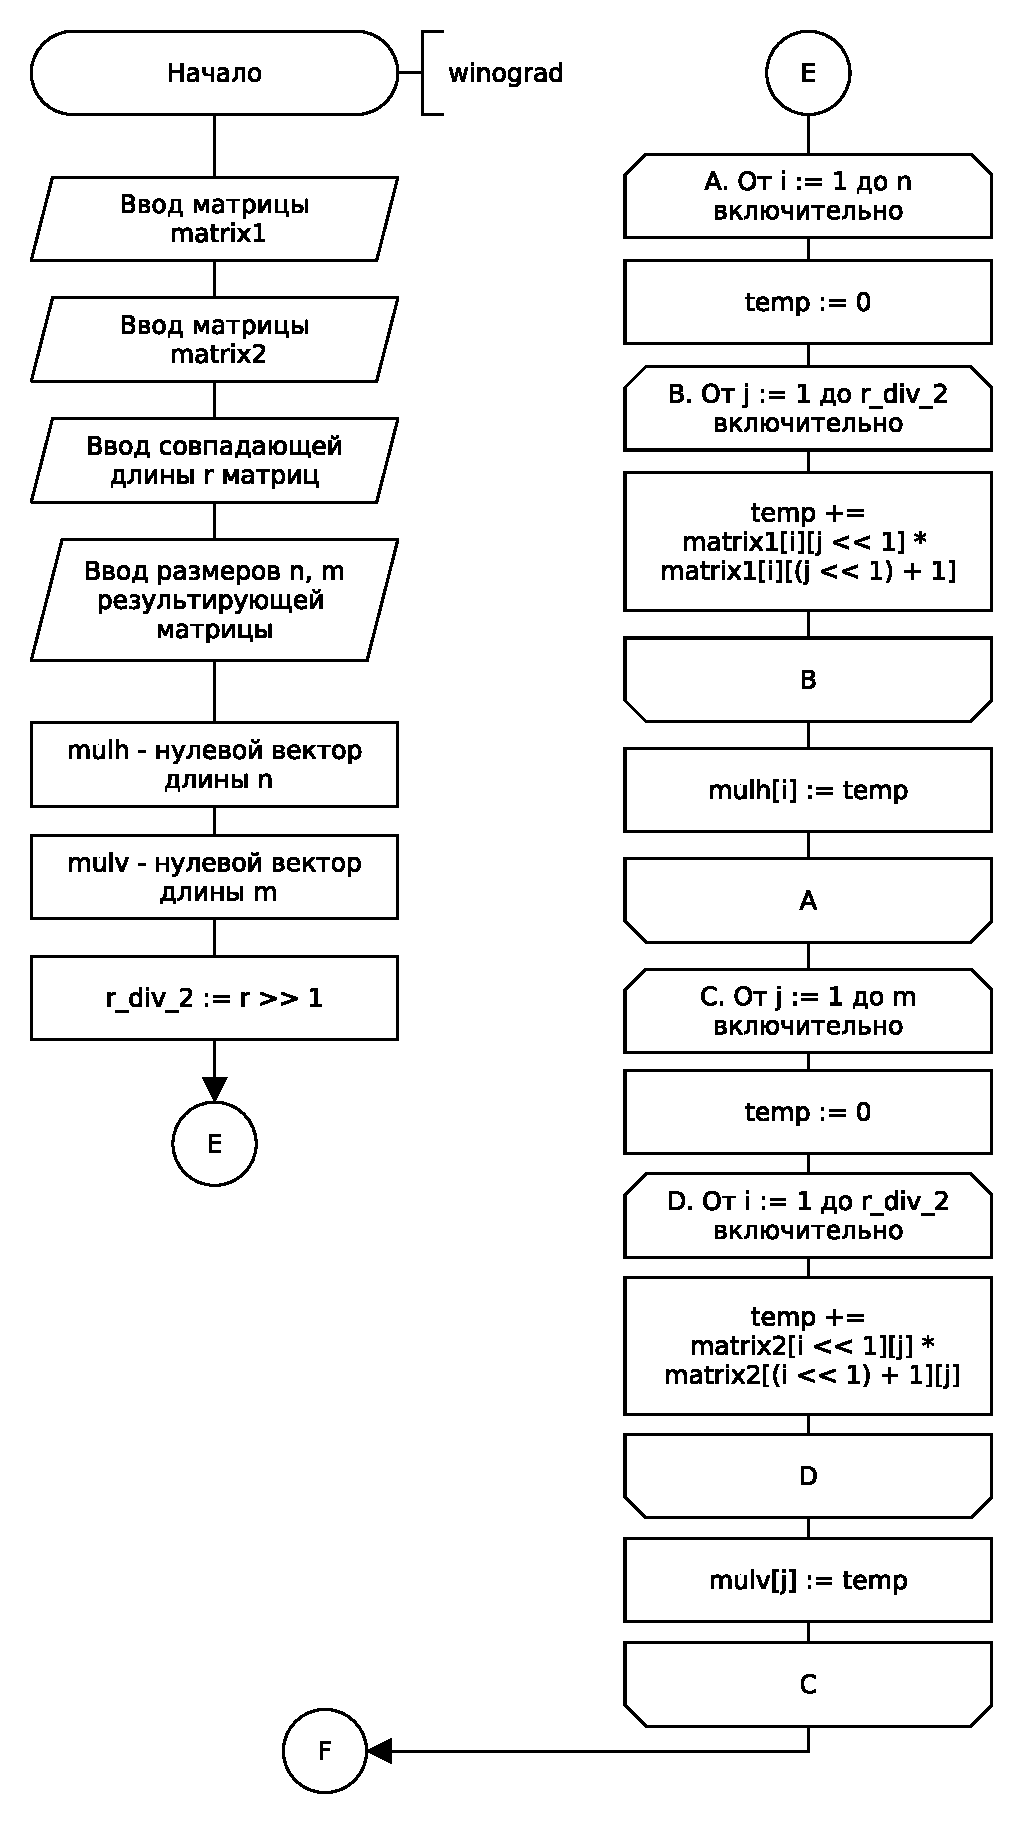
\includegraphics[scale=0.70]{pdf/owinograd-part1.pdf}
    \caption{Алгоритм Винограда, часть 1}
    \label{img:windograd1}
\end{figure}

\begin{figure}[H]
    \centering
    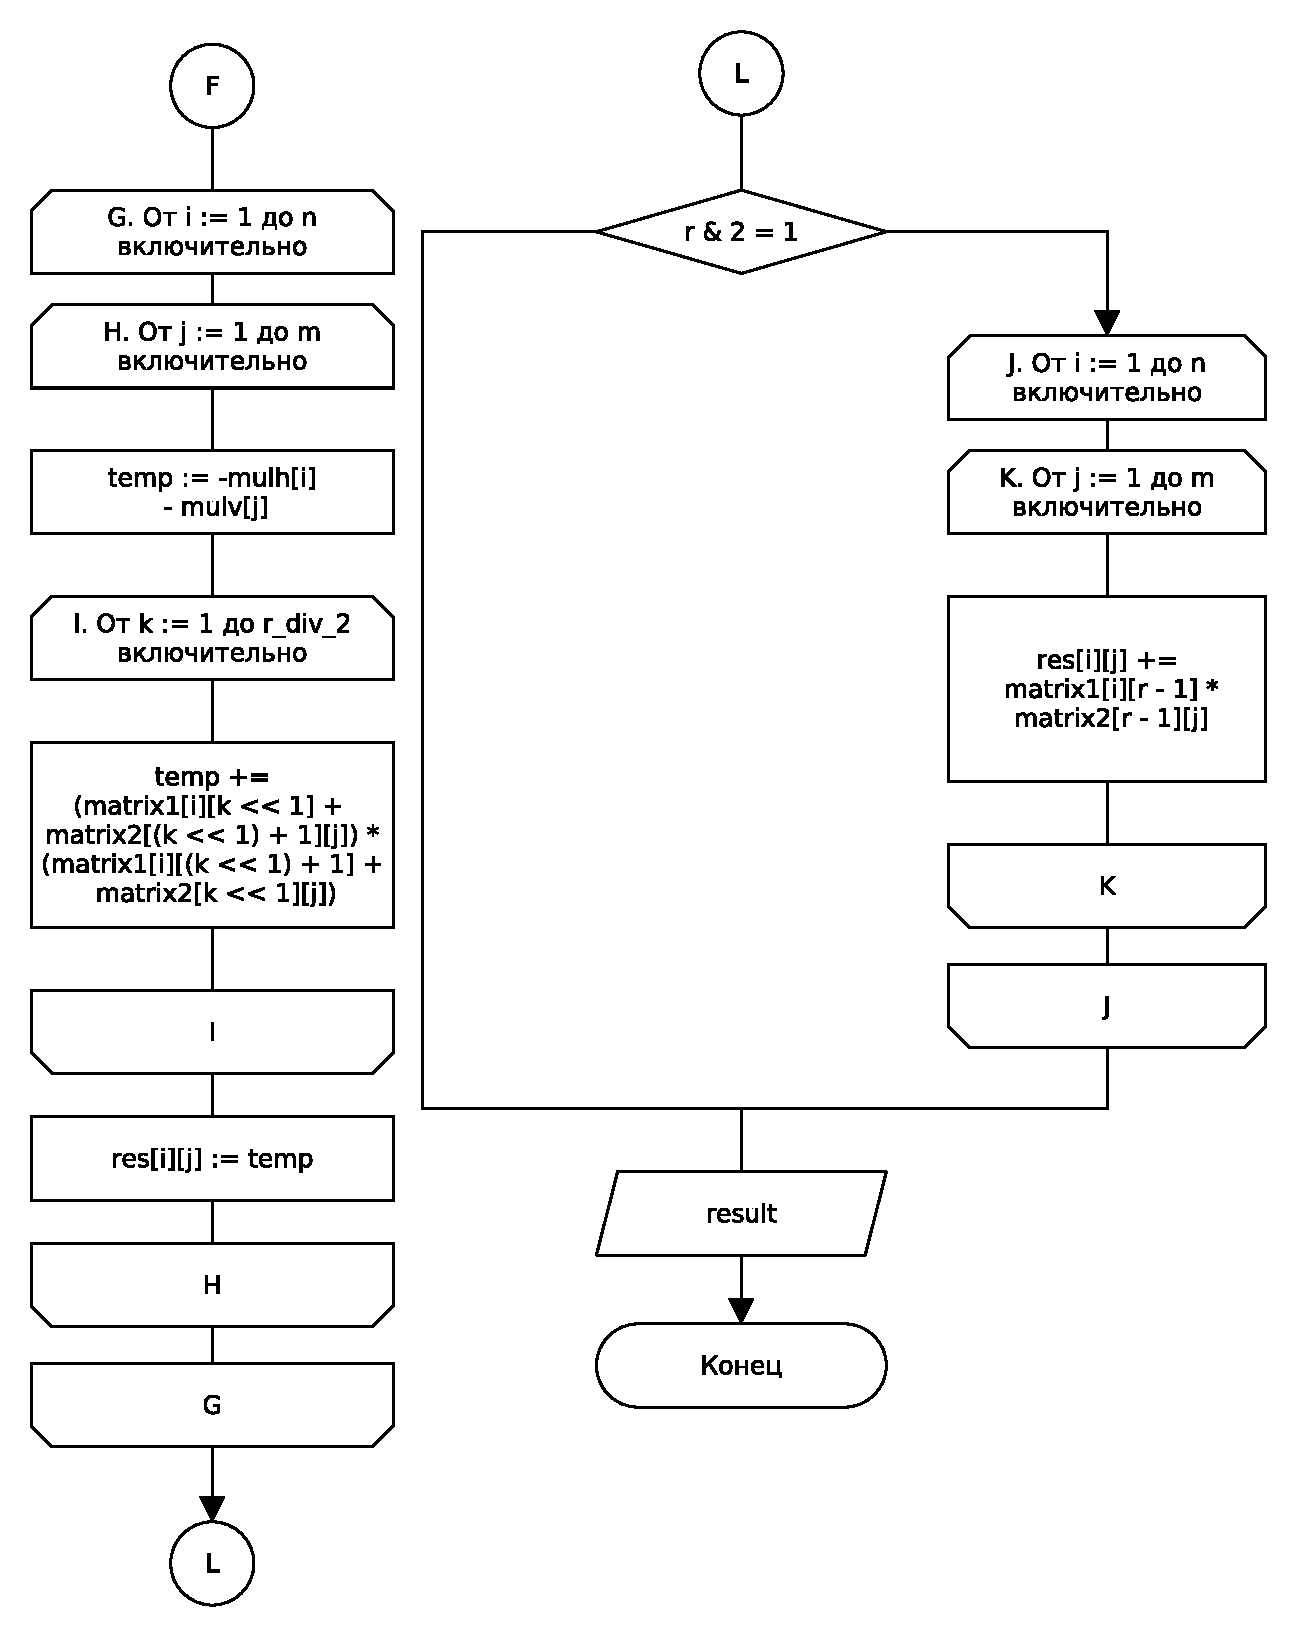
\includegraphics[scale=0.70]{pdf/owinograd-part2.pdf}
    \caption{Алгоритм Винограда, часть 2}
    \label{img:windograd2}
\end{figure}

\subsection{Параллелизированный алгоритм Винограда}

Пусть, даны две матрицы: матрица 1 и матрица 2. Разобьём матрицу 1 построчно на столько подматриц, сколько потоков используется при распараллеливании. Тогда результат умножения матрицы 1 на матрицу 2 будет равен объединению произведений подматриц матрицы 1 на матрицу 2 в порядке их разбиения. На рисунке \ref{img:pwindograd} изображён параллелизированный алгоритм Винограда, основанный на обычном.
\begin{figure}[H]
    \centering
    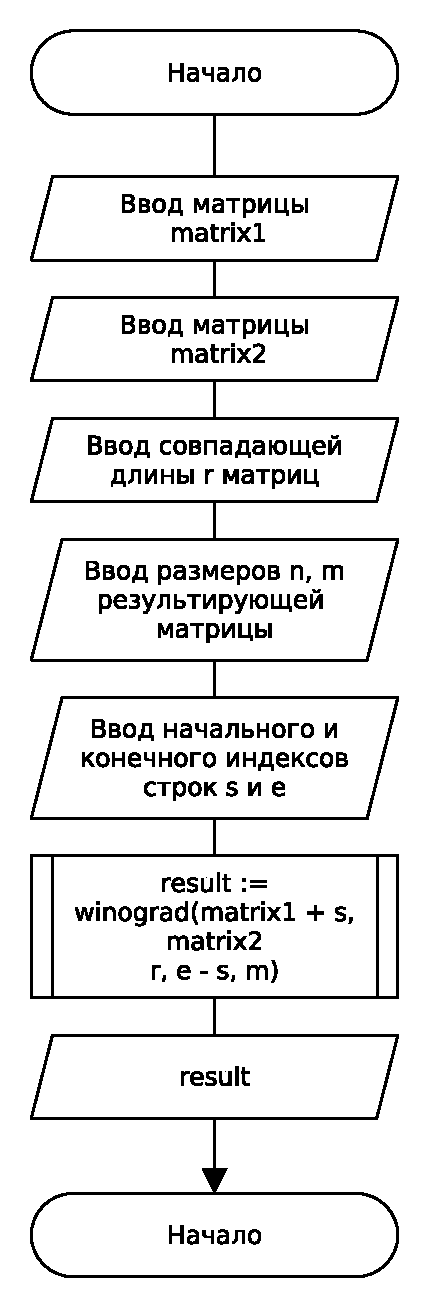
\includegraphics[scale=0.70]{pdf/pwinograd.pdf}
    \caption{Параллелизированный алгоритм Винограда}
    \label{img:pwindograd}
\end{figure}

\section{Вывод}
Благодаря тому, что вычисление каждого элемента матрицы произведения независимо от остальных, удалось разработать параллелизированный алгоритм Винограда.

